\documentclass{article}
% \usepackage{doc}
% \usepackage{ltxcmds}
\usepackage{graphicx} % Required for inserting images
\usepackage{algorithm}
\usepackage{algorithmic}
% \usepackage{algpseudocode}
% \usepackage{multicol}
\usepackage{xcolor}
% \usepackage{soul}
% \usepackage[left=1.5cm,right=1.5cm]{geometry}
% \usepackage{verbatim}
% \usepackage{multirow}
% \usepackage{tikz}
% \usepackage{url}
\usepackage{amsthm} % FOR THE PROOF ENVIRONMENT
                    % (MAYBE IT BUYS US OTHER THINGS TOO)
% REDO THE ENVIRONMENTS RIGHT
\newtheorem{definition}{Definition}
\newtheorem{example}{Example}
\newtheorem{remark}{Remark}
\newtheorem{theorem}{Theorem}
\newtheorem{lemma}{Lemma}
\newtheorem{corollary}{Corollary}
%\newtheorem{conj}{Conjecture}
\newtheorem{proposition}{Proposition}

% using soul just for setstcolor is overkill, soul is for
% many other things and that one is easily circumvented
% \setstcolor{red}  % tachado rojo
% \newcommand{\deleted}[1]{\st{#1}}        % rojo

\newcommand{\added}[1]{\textcolor{blue}{#1}}
\newcommand{\deleted}[1]{\textcolor{red}{#1}}
\newcommand{\replaced}[2]{\deleted{#2}\ \added{#1}}
%~ \newcommand{\added}[1]{{#1}}
%~ \newcommand{\deleted}[1]{{#1}}
%~ \newcommand{\replaced}[2]{\deleted{#2}\ \added{#1}}

% REPLACED BY ABOVE
% \usepackage{soul}
% \setstcolor{red}  % tachado rojo
% % Macros compatibles con tu flujo
% \newcommand{\added}[1]{\textcolor{blue}{#1}}          % azul
% \newcommand{\deleted}[1]{\st{#1}}        % rojo
% \newcommand{\replaced}[2]{\deleted{#2}\ \added{#1}}
\newcommand{\st}[1]{%
  \sbox0{#1}%
  \usebox0%
  \llap{\rule[0.5ex]{\wd0}{0.4pt}}%
}

\renewcommand{\floatpagefraction}{0.7} % FOR THE LATTICE NOT GETTING ALONE

% LIPIcs FORMATTED AND SO - SKIP TO BELOW FOR NONFORMATTED
%This is a template for producing LIPIcs articles. 
%See lipics-v2021-authors-guidelines.pdf for further information.
%for A4 paper format use option "a4paper", for US-letter use option "letterpaper"
%for british hyphenation rules use option "UKenglish", for american hyphenation rules use option "USenglish"
%for section-numbered lemmas etc., use "numberwithinsect"
%for enabling cleveref support, use "cleveref"
%for enabling autoref support, use "autoref"
%for anonymousing the authors (e.g. for double-blind review), add "anonymous"
%for enabling thm-restate support, use "thm-restate"
%for enabling a two-column layout for the author/affilation part (only applicable for > 6 authors), use "authorcolumns"
%for producing a PDF according the PDF/A standard, add "pdfa"

%\pdfoutput=1 %uncomment to ensure pdflatex processing (mandatatory e.g. to submit to arXiv)
%\hideLIPIcs  %uncomment to remove references to LIPIcs series (logo, DOI, ...), e.g. when preparing a pre-final version to be uploaded to arXiv or another public repository

%\graphicspath{{./graphics/}}%helpful if your graphic files are in another directory

% \bibliographystyle{plainurl}% the mandatory bibstyle
% \title{Enumerating Closed Sets in Order of Descending Support} 
% \titlerunning{Closed Sets in  Descending Support} %TODO optional, please use if title is longer than one line
% \author{Jos\'e Luis Balc\'azar\footnote{Optional footnote, e.g. to mark corresponding author}}{    Departament de Ciències de la Computació, Universitat Politècnica de Catalunya, C/ Jordi Girona Salgado 1-3, Edif. Omega-K2M, 08034 Barcelona, Spain }{jose.luis.balcazar@upc.edu}{https://orcid.org/0000-0003-4248-4528}{(Optional) author-specific funding acknowledgements}%TODO mandatory, please use full name; only 1 author per \author macro; first two parameters are mandatory, other parameters can be empty. Please provide at least the name of the affiliation and the country. The full address is optional. Use additional curly braces to indicate the correct name splitting when the last name consists of multiple name parts.
% \author{Cristina T\^irn\u{a}uc\u{a}}{Departmento de Matemáticas, Estadistica y Computación, Universidad de Cantabria, Av. de los Castros, 39005, Santander, Spain}{cristina.tirnauca@unican.es}{[https://orcid.org/0000-0002-7129-2237]}{This work has been partially supported by grants PID2022-139237NB-I00 and PID2023-146243OBI00 funded by MICIU AEI/10.13039/501100011033 and by ERDF/EU}
% \authorrunning{José Luis Balcázar and Cristina T\^irn\u{a}uc\u{a}} %TODO mandatory. First: Use abbreviated first/middle names. Second (only in severe cases): Use first author plus 'et al.'
% \Copyright{José Luis Balcázar and Cristina T\^irn\u{a}uc\u{a}} %TODO mandatory, please use full first names. LIPIcs license is "CC-BY";  http://creativecommons.org/licenses/by/3.0/
% \ccsdesc[100]{\textcolor{red}{Replace ccsdesc macro with valid one}} %TODO mandatory: Please choose ACM 2012 classifications from https://dl.acm.org/ccs/ccs_flat.cfm 
% \keywords{Pattern mining, closure mining, itemset support} %TODO mandatory; please add comma-separated list of keywords
% \category{} %optional, e.g. invited paper
% \relatedversion{} %optional, e.g. full version hosted on arXiv, HAL, or other respository/website
%\relatedversiondetails[linktext={opt. text shown instead of the URL}, cite=DBLP:books/mk/GrayR93]{Classification (e.g. Full Version, Extended Version, Previous Version}{URL to related version} %linktext and cite are optional

%\supplement{}%optional, e.g. related research data, source code, ... hosted on a repository like zenodo, figshare, GitHub, ...
%\supplementdetails[linktext={opt. text shown instead of the URL}, cite=DBLP:books/mk/GrayR93, subcategory={Description, Subcategory}, swhid={Software Heritage Identifier}]{General Classification (e.g. Software, Dataset, Model, ...)}{URL to related version} %linktext, cite, and subcategory are optional

%\funding{(Optional) general funding statement \dots}%optional, to capture a funding statement, which applies to all authors. Please enter author specific funding statements as fifth argument of the \author macro.

% \acknowledgements{I want to thank \dots}%optional

%\nolinenumbers %uncomment to disable line numbering

% {Closed sets enumeration in descending support: 
% comparison of existing algorithm and a new proposal }


%Editor-only macros:: begin (do not touch as author)%%%%%%%%%%%%%%%%%%%%%%%%%%%%%%%%%%
% \EventEditors{John Q. Open and Joan R. Access}
% \EventNoEds{2}
% \EventLongTitle{42nd Conference on Very Important Topics (CVIT 2016)}
% \EventShortTitle{CVIT 2016}
% \EventAcronym{CVIT}
% \EventYear{2016}
% \EventDate{December 24--27, 2016}
% \EventLocation{Little Whinging, United Kingdom}
% \EventLogo{}
% \SeriesVolume{42}
% \ArticleNo{23}
%%%%%%%%%%%%%%%%%%%%%%%%%%%%%%%%%%%%%%%%%%%%%%%%%%%%%%


\def\U{\mathcal{U}}
\def\C{\mathcal{C}}
\def\s{\mathit{s}}
\newcommand{\cl}[1]{\overline{#1}}
\def\bef{\prec} 

% \begin{document}

% \maketitle

\title{A Decreasing-Support Variant of a Classical Linear Time Closure Miner}
\author{Jos\'e Luis Balc\'azar, Cristina T\^irn\u{a}uc\u{a}}
\date{September 2026}

\begin{document}

\maketitle

\begin{abstract}
In applications developing data analysis on 
transactional datasets, one common intermediate 
step is the computation of so-called closed sets. 
To our knowledge, the earliest linear time algorithm
for this task was devised by Ganter in 1984.
The family of closed sets being often far too large, 
it is common to impose a lower bound on their support, 
that is, on how frequent they are to be; in practice, 
however, we lack reliable hints as to how to choose 
the threshold.
One alternative proposal is to enumerate the 
closed sets in order of descending support, 
so as to stop the enumeration when sufficient 
information has been gathered: as if the threshold 
had been set from the start at the point where the 
algorithm is stopped.
We show here modifications to Ganter's algorithm that 
achieve this goal.
\end{abstract}


\section{Introduction}
\label{sec:Intro}


We consider variations of algorithms that obtain closed 
sets out of a closure operator on finite sets. In many
applications, the closure operator is defined in terms
of a transactional dataset (or, equivalently, a so-called
formal context). While most closed-set-based data analysis 
developments could conceivably operate on all closed sets, 
most often only frequent closed sets, for some support
lower bound, are considered, given the large amounts of 
closed sets usually arising from even smallish datasets. 
In these cases, the family of closed sets acts in fact
as one of several notions of condensed representations 
of the family of all frequent sets since all the relevant
informantion can be recovered from their supports.
A survey on condensed representation for frequent sets 
is \cite{CaRiBo05}. Books and surveys such as 
\cite{CegRod06,GanWil99,GenHam06} 
are helpful to trace further literature if necessary.

One of the difficult aspects of practical work with frequent
closed sets, whether on themselves or as a stepping stone
for other processes, is the lack of practically successful
criteria for setting the support threshold. Whereas there 
are real-life datasets for which one has to fix a threshold 
below 1\% in order to find any frequent closed set at all, there are 
others where a strict threshold of 95\% is already impractical 
in that it gives rise to hundreds of thousands of closed 
frequent sets. Besides, it is often the unexperienced end user 
of the application that has to deal with the problem of adjusting 
the support just right. 

Several references propose variations of algorithms that, if let 
run to the end, would enumerate in order of decreasing support 
all the closed sets, but allow the user to interrupt the search 
when either a sufficient number of closed sets has been found 
or the ``patience'' resource has been exhausted. 
This note focuses on one specific algorithm,
\textsc{NextClosure}, that allows one to construct
the family of closed sets in time linear in the length
of the family~\cite{Gant10}\footnote{Specifically, 
the earliest algorithm to our knowledge to match 
that description: the 2010 publication \cite{Gant10} 
is, in fact, a facsimile that clearly displays the 
original date of 1984.}.
We aim at variants that, if applied to a closure space 
obtained from a dataset, would return the closed sets in
order of decreasing support. While the algorithmic look
will not vary by much, the mathematics that validate the
key decisions to accelerate the process are far from 
trivial and worthy of a focused note (this one).
Comparisons with other algorithms
that list closed sets in order of decreasing support (such as
the one implicit in one of the theorems of \cite{boros2003maximal},
the one employed in the open-source tool \textsc{yacaree}
and the proposal in \cite{pietracaprina2007efficient} of a
support-decreasing variant of the Linear-time Closure Miner (LCM) 
algorithm of \cite{UAUA04}) are, for the time being, postponed 
to a longer text in preparation. We just advance that extensive
experimentation leaves no clear winner but does reduce the 
considerations to a small head group, in which our own contribution 
is a contender.

\added{Most urgent: unify the names of items along all the algorithms.
Right now our Ganter uses $x_i$ in the loop and $j < i$ for the test,
our Yacaree (in case it remains here) uses $a_j$ in the loop and 
our Troppus-0 uses $a_j$ in the loop and $i < j$ for the test. 
No way to understand anything.
What is the good choice? Ganter himself used directly integers $i$
as items thus sparing indexitis.}

\section{Preliminaries}\label{sec:Prel}

\added{Pending definitions: closure? support? $X$ \emph{comes before} $Y$,
denoted $X\bef Y$? lectic ordering? (can we do without? but we need 
a tie-breaking criterion anyway for coinciding supports)
I would like to reduce the number of involved notions and notations
to the bare minimum. --JLB}

Ganter's \textsc{NextClosure} algorithm is described as 
Algorithm~\ref{alg:Ganter}; it takes the form of an algorithm 
to obtain, from a given closure, a ``next'' one. Its author 
provided mathematical guarantees that prove that, starting 
with the closure of the empty set, repeated application of 
\textsc{NextClosure} will traverse completely and without 
repetition the whole family of closed sets. Equivalently, 
the binary relation between the input and the output closures, 
seen as a graph on the family of all closed sets, is a path 
connecting all of them with no branching or loops.

\added{This last sentence is intended to start alluding to
the future perspective of "gating". --JLB}

\begin{algorithm}
  \caption{Ganter's \textsc{NextClosure}}\label{alg:Ganter}
  \begin{algorithmic}[1]
  	  \STATE Given: $X$ (the current closure)
    	\FOR {$i = m,m-1,\ldots,2,1$ }
    		\IF {$x_i \notin X$}
            \STATE $Y = \cl{X  \cap \{x_1,x_2,\ldots,x_{i-1}\} \cup \{x_i\}}$
            \IF{$\forall x_j \in Y $ con $j<i$, $x_j \in X$}
             
      		\RETURN $Y$ (the next closure)
            \ENDIF
         \ENDIF
      \ENDFOR
  \end{algorithmic}
\end{algorithm}


\added{Preserve something of the next paragraphs? --JLB}

The way we chose to describe our
algorithm is on the basis of the approach from~\cite{Gant10}, 
which is also the lesser
known (being the older notwithstanding), because it allows for a
simpler ``local'' view of the process by concentrating only on
two closures at a time: the current one, $X$, and how to obtain the next.

We give it in Algorithm~\ref{alg:Ganter}.~Essentially, 
the key point is in an auxiliary operation of adding 
an item to an itemset: 
simultaneously, one removes all smaller elements;
then, the closure of
the new itemset is found, and is deemed acceptable if it did not add
any item that would be considered at a later loop. The smallest item
leading to an acceptable closure leads to the next closure according
to the lectic ordering, defined below. We are actually reversing the 
item ordering from \cite{Gant10} in order to better compare to our 
contribution below.

(Here, and along the paper, 
$Y\backslash X$ denotes the items of $Y$ 
that do not belong to $X$.)

\added{Can we do without the backslash operator? --JLB} 

\section{Decreasing-support variants}\label{sec:Main}

\added{Consider starting this section with the description 
of the yacaree algorithm. Copied here just in case. --JLB}

The yacaree option... unpublished so far as algorithm but 
available as open source... basically we add the closures to a heap...
careful that here items seem to be $a_i$ while 
in our description of Ganter they were $x_i$
(and in the original in Ganter just $i$).


\begin{algorithm}
\caption{{\sc Yacaree}} % \label{algorithm}
  \begin{algorithmic}[1]
    \STATE $h = \{\overline{\emptyset}\}$ \COMMENT{add closure of $\emptyset$ to an empty heap}
    \WHILE {$h$ not empty} 
    	\STATE $X = h$.pop() \COMMENT{minimal element from the heap $h$}
        \STATE yield $X$
    	\FOR {$a_j$ in $\{a_1,\ldots,a_n\}  \backslash X$}
    		\STATE $Y=\overline{X \cup \{a_j\}}$
    		  \IF {$Y$ not in $h$}
    		  	\STATE add $Y$ to $h$
        	\ENDIF
      \ENDFOR

    \ENDWHILE
  \end{algorithmic}
\end{algorithm}

Essentially, this algorithm  operates as follows: 
closures ``pending to expand'' are kept in a heap, 
which provides us efficiently with the pending closure of highest 
support; then this closure is extended by adding items and applying
closures to obtain new pending closures that are added to the heap.
There is an internal support bound that starts low (can start at~1)
and is increased along the way when the growth of the heap threatens
to overflow the memory. Of course, the main issue to be dealt with
is that of avoiding repetitions, which is done via a rather basic
but still considerably efficient hashing scheme. 

\added{Attempt at right-to-left version of current Troppus follows. 
But here $\U$ is formed by $x$'s and in the algorithms by $a$'s. --JLB}

Let $\U=\{x_1,\ldots,x_n\}$ be the set of items in order of 
% \deleted{descending} 
\emph{ascending} support, i.e., 
for all $1 \leq i < j \leq n$ we have $\s(x_i) \leq \s(x_j)$. 
Note that supports, and therefore the ordering in $\U$, depend 
on the dataset. One can easily count the support of all singletons 
in a single traversal of the dataset and, then, sorting them requires 
$\mathcal{O}(n \log n)$ time steps. For the items having the same 
support the order can be fixed arbitrarily. 

\added{However, for the example below, the itemsets $ae$ and $be$ 
have the same support and we should take care that whatever order 
they are reported in by the algorithm does not puzzle the reader, 
who will be puzzled enough by the intricacies of the proof. --JLB}

Being much in the spirit of \textsc{NextClosure}, our variant
is reasonably simple. 

\added{Propondré llamarlo de otra manera. Lo comentaremos.
Entre nosotros, de momento, Troppus-0. --JLB}

We call our algorithm \textsc{Troppus}, 
that is, \textsl{support} read backwards to remind of the
decreasing-support ordering condition.

The intuitions are as follows. 

\added{I believe now that all these paragraphs of "intuitions" 
do more to confuse the reader than to enlighten her/him. --JLB}

We try to apply
the efficient linear-time traversal. Of course, often, the
support values will make it impossible to stick to it.
As in the yacaree closure miner, we keep 
a heap $h$ of some closures that still must be
enumerated in the future; 
each of them will allow us to possibly traverse 
further closures in  lectic order. Hence, the purpose of the
heap is not to store all pending closures
but only to keep track of segments where
there is a disagreement between decreasing-support
ordering and lectic ordering.

Thus, at each main loop we pick up the next closure $X$
from the heap: ``minimal'' according to 
the ``comes before'' ordering. 
For this to work, the support is to be stored jointly with the
closure in the heap, but we will not make this fact
explicit in the algorithm yet, for the sake of clarity.
It will be clear in the example below.

On this $X$, we apply a process similar to the one in \textsc{NextClosure},
except that here we cannot be satisfied with one single step:
it depends on whether the lectic ordering and
the decreasing-support ordering match. As this is not 
guaranteed, we expand with all possible items in turn,
in order of decreasing support.
As in \textsc{NextClosure}, closures that add too 
small elements are discarded; we will revisit these 
closures later, in due time, thanks to those smaller 
elements.

We will argue
the following: given two extensions of $X$ with 
different items $x$ and $y$,
where $x\bef y$, if the support obtained 
extending with $y$ is less than extending with $x$,
we do not need to care for it: it agrees enough with the
lectic ordering and will be picked up again. But, if it
is more, we will need to remember both,
as the lectic ordering will not
go back and pick up the extension with $x$ after visiting
that with $y$. Of course, these statements are
not self-evident, and are indicated here just as explanation:
formal proofs are given below.

Thus, we maintain a ``local list'' $l$ of itemsets that
we must keep: those extensions that lead to higher support
than the previous ones even though the item which is used 
to trigger the extension has lower support as singleton.

As a consequence, closures already visited may be 
hit again later. If the next step should lead us to
higher support, we just abandon the expansions process
as it and all the remaining ones have been already treated earlier.

All this can be gathered formally in the following algorithm. Here we
employ the shorthand ``report $X$'' to indicate that a new closure $X$
has been found. It would be implemented by adding it to a list of 
closures, or by ``yielding'' it on to further processing if that sort
of iterators are available in the programming platform 
(see \cite{BaGaDe12}). % Balcazar/Garcia-Saiz/delaDehesa

\added{In the source, the algorithm is here, but it will
probably float away to the next page and the text should
take that into account. --JLB}

\begin{algorithm}
\caption{\textsc{Troppus}}\label{algorithm}
  \begin{algorithmic}[1]
    \STATE $h = \{\overline{\emptyset}\}$ \COMMENT{add closure of $\emptyset$ to the global list $h$, an empty heap}
    \WHILE {$h$ not empty} 
    	\STATE let $X$ be the closure of maximum support from the heap $h$
    	\STATE report $X$
    	\STATE define an empty list $l$ \COMMENT{the local list}
    	\STATE set $m=0$
    	\COMMENT{loop in order of decreasing support}
    	\FOR {$a_j$ in $\{a_n,\ldots,a_1\}$} 
	  		\IF {$a_j \notin X$}
	  		    \STATE $Y = (X \cap \{a_1,\ldots,a_{j-1}\}) \cup \{a_j\}$
	  		    \STATE check the following 3 conditions on its closure $\cl{Y}$:
    		  		\IF {(Condition 1) $\s(Y) = s(\cl{Y}) > \s(X)$}
    					\STATE break \COMMENT{for-loop ends, nothing added further to $l$}
    				\ENDIF
    		  		\IF {(Condition 2) $\exists a_i \in \cl{Y} (i < j \land a_i \notin X)$ 
    		  		\OR (Condition 3) $(\s(Y) \leq  m)$}
      					\STATE continue \COMMENT{move on to the next item in the for loop}
    				\ENDIF
					\STATE append $\cl{Y}$ to $l$
					\STATE set $m = \s(Y) = s(\cl{Y})$
			\ENDIF
		\ENDFOR
		\STATE add to $h$ the elements of $l$
    \ENDWHILE
  \end{algorithmic}
\end{algorithm}

Together with the updating of $m$ when a closure enters the local
list $l$, Condition (3) means that subsequent additions to the local 
list enter it with increasing supports.
This is where the sophistication of this algorithm lies:
at face value, there is no reason for that condition hitting the
``sweet spot'' where no repeated closures are added ever to the 
heap while ensuring that all of them are added at some point. 
We return to this fact in the mathematical proofs below.

Condition (1) stops the loop: the current closure $\cl{Y}$ has been
already visited before, due to the decreasing support condition,
as are all those possible additions to the local list because
Condition (3) would ensure them to be already visited as well.

Condition (2) is fully analogous to the one applied by Ganter and
plays a similar role; we still must ensure that it does also in the
new context.

The local list $l$ will facilitate our mathematical validation
of the algorithm. However, note that $h$ is made as the successive
unions of local lists; and that neither $h$ nor $l$ are \emph{consulted}
during the loop. Hence, in our implementation, the elements of the
local list go directly into the heap instead. We write the algorithm
so as to have a name ready for the batch of closures
that get added to the heap upon processing $X$, as this notation will
be important in the validation.

\subsection{A Complete Example}\label{sec:Example}
We believe that running our algorithm on an example could provide the 
reader with some insight into the way it works. 

\added{We will also use this example to point out some implementation 
details that we chose not to include into the algorithm's description 
in order not to obscure its validation which is already quite 
intricate. NOT true anymore, I believe, I moved them out. --JLB)}

So let us consider again the dataset from Example \ref{example}.
There are a total of 12 closed sets: $\emptyset_{/24}$, $a_{/12}$, 
$b_{/11}$, $cd_{/10}$, $e_{/9}$, $ab_{/6}$, $ae_{/5}$, $be_{/5}$, 
$cde_{/4}$, $bcde_{/3}$, $abe_{/2}$, $abcde_{/1}$. The bar and 
subindex mark the support of each itemset. The associated lattice 
is shown in Figure \ref{fig:lattice}. 


\begin{figure}[t]
\begin{center}
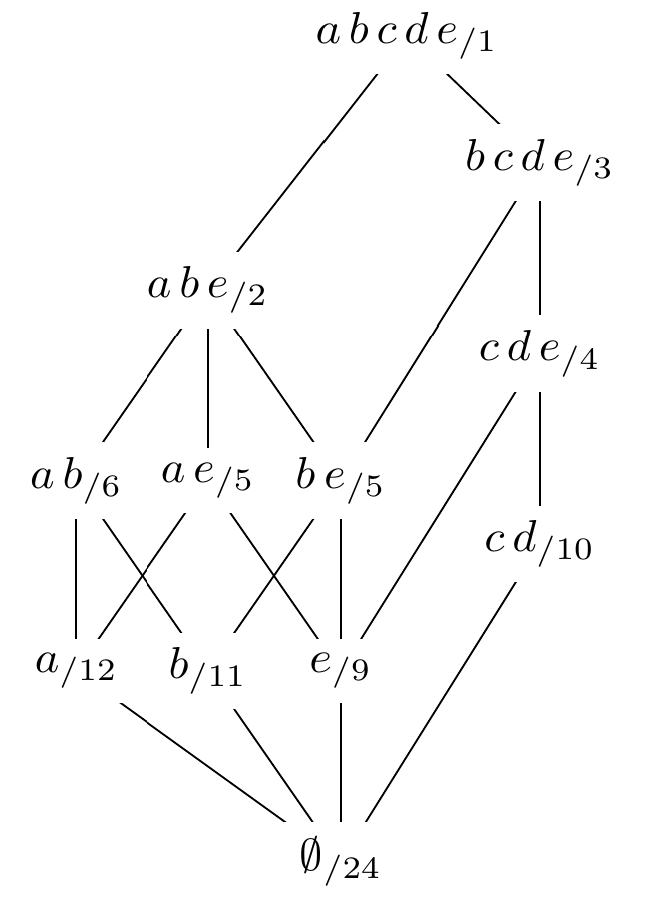
\includegraphics[height=0.4\textheight]{lattice24.png}
\caption{A lattice of closures}\label{fig:lattice}
\end{center}
\end{figure}


During the run of the algorithm, some of the closures 
computed will be added to the local list, and some others 
will be discarded, either because
% 
  their support is larger than the support of the 
  current working closure $X$ (\textsl{Condition~1}), 
or 
  because they have added to the closure some element 
  smaller than the current working item $x$ 
  (\textsl{Condition 2}), 
or
  because they would not comply with the increasing 
  support along the local list (\textsl{Condition 3}). 

In the first case, the for loop is 
%forcibly %look for an alternative adverb or use no adverb
abandoned and no further items are visited 
for the current working itemset $X$. 

\added{These two paragraphs are fully general. Maybe
the example is not the right place for them.}

In the sequel we give, for each closed set $X$, 
a detailed explanation of how the local list is 
generated. Thus, one may check that the closures 
are returned in the desired order.

\begin{itemize}
\item $X=\emptyset$: the algorithm tries all 
items $x$ in $\U$ and computes five closures by
considering items in order of decreasing support:
$\textbf{a}$, $\textbf{b}$, $\textbf{c}\underline{d}$, 
$\underline{c}\textbf{d}$ and $\textbf{e}$. 
We will represent in boldface the current item, 
and underline the items added by the closure operator. 
The first closure $a$ meets all conditions, so it gets 
to be added to the local list, while the value of $m$ 
is updated to $\s(a)=12$. All other closures will 
therefore fail Condition 3, so $l=[a]$ and $h=[a_{/12}]$.
Note that $\textbf{c}\underline{d}$ fails also
Condition 2 because $d < c$ was added by the closure 
operator; but no case fails Condition 1.

\item $X=a$: $x$ takes, in turn, the values $b, c, d, e$
so four closures are generated: $\textbf{b}$, 
$\textbf{c}\underline{d}$, $\underline{c}\textbf{d}$, 
$\textbf{e}$, and only the first one is added to $l$ 
because the others have strictly smaller support and 
fail Condition 3. Thus, $l=[b]$ and $h=[b_{/11}]$. 
The observation about $\textbf{c}\underline{d}$ 
applies again.

\item $X=b$: $x$ takes, in turn, the values $a, c, d, e$ 
and the following closures are computed: $\textbf{a}b$
(note that $b\in X$ and $\s(a) > \s(b)$ so that $b$ 
is neither boldface nor underlined), 
$\textbf{c}\underline{d}$, $\underline{c}\textbf{d}$, 
$\textbf{e}$. The algorithm adds to the local list 
the first and the third: the second fails Condition 2
as before and the fourth one does not meet Condition 3 
about increasing support. Therefore, 
$l=[ab, cd]$ and $h=[ab_{/6}, cd_{/10}]$. 

\item $X=cd$: $x$ takes, in turn, the values $a, b, e$. 
The algorithm generates three closures: 
$\textbf{a}\underline{b}cd\underline{e}$, 
$\textbf{b}cd\underline{e}$, $\textbf{e}$. 
The first two are not added to the local list because 
they fail Condition 2 (note that $e$ is smaller than 
both $a$ and $b$). So, $l=[e]$ and $h=[ab_{/6}, e_{/9}]$.

\item $X=e$: the following closures are generated: 
$\textbf{a}e$, $\textbf{b}e$, $\textbf{c}\underline{d}e$ 
and $\underline{c}\textbf{d}e$, and only the first one is 
kept, since the other ones have support smaller than or 
equal to $\s(ae) = 5$ and thus fail Condition 3
(and also Condition 2 in the same usual case). 
Hence, $l=[ae]$ and $h=[ab_{/6}, ae_{/5}]$. \added{Ahora que 
"el orden va al revés", el criterio que teníamos sobre cómo
desempatar y la definición que usábamos de "comes before"
creo que requeriría que el desempate en soporte 5 se
resolviera al revés de como lo resolvemos. De momento,
por esa razón preferiría evitar el "comes before".}

\item $X=ab$: for $x=c$, the closure obtained, 
$\textbf{c}\underline{d}$, does not get to the local list 
by Condition 2 as before. But, for $x=d$, the closure is 
the same, $\underline{c}\textbf{d}$, but this time it would be 
admissible because $c$, the element added by the closure 
operator, is larger than the current working item $d$. 
Nevertheless, it fails Condition 1: $\s(cd)=10>6=\s(ab)$.
Not only it does not get to be added to the local list, 
which is necessary to avoid repetitions since it was
already covered before; it even forces the loop to exit 
and blocks further items from being visited. Thus, $l$ 
remains empty and $h=[ae_{/5}]$. The closure $abe$
blocked by exiting the loop will be picked up again 
later.

\item $X=ae$: $x$ takes, in turn, the values $b, c, d$ 
and the algorithm generates three closures $\textbf{b}e$, 
$\textbf{c}\underline{d}e$ and $\underline{c}\textbf{d}e$. 
Since $\s(cde)=4 \leq 5=\s(be)$, the last two of them both 
fail Condition 3, so $l=[be]$ and $h=[be_{/5}]$. 

\added{Here we had this sentence but I believe it is 
wrong now: Note that $ae$ comes before $be$ even though 
$\s(ae)=\s(be)=5$ since $ae$ is lectically smaller than $be$.}

\item $X=be$: the closures generated are $\textbf{a}be$, 
$\textbf{c}\underline{d}e$ and $\underline{c}\textbf{d}e$. 
The second one fails Condition 2 as usual, but the first 
and the third do get added to the local list. Hence, 
$l=[abe, cde]$ and $h=[abe_{/2}, cde_{/4}]$.

\item $X=cde$: among the generated closures, 
$\textbf{a}\underline{b}cde$ and $\textbf{b}cde$, 
only the second one gets to be added to the local list 
since the first one fails Condition 2. 
Thus, $l=[bcde]$, $h=[abe_{/2}, bcde_{/3}]$.

\item $X=bcde$: only one set is generated, 
$\textbf{a}bcde$, and subsequently added to 
the local list. So, $l=[abcde]$ and $h=[abe_{/2}, abcde_{/1}]$.

\item $X=abe$: none of the generated closed sets,
$\textbf{c}\underline{d}e$ and $\underline{c}\textbf{d}e$, 
make it to the local list: the first one fails Condition 2
again and the second one, although this time does meet 
Condition 2 (note that it is the same closure with 
different working item), fails Condition 1 since its 
support is bigger than $\s(abe)$. Thefore, $l=[]$ and 
$h=[abcde_{/1}]$.

\item $X=abcde$: nothing more is generated and the 
algorithm stops, with $l=[]$ and $h=[]$.
\end{itemize}


\added{The next paragraph is out of place. --JLB}

As an additional remark, we mention that we have found slightly more
efficient to decouple the computation of $s(Y)$ from the computation 
of $Y$ itself, more precisely from the closure operator. In our
implementation, we construct $X \cup \{x\} \backslash \{y \in X \mid y < x\}$,
evaluate its support, test it against $m$, and only then compute the
closure and proceed with the algorithm. This spares some running time,
although only to a rather minor extent. 

\added{Comments that were inserted into the example:
(In our implementation of the algorithm we actually test for support before computing the closure - a small technicality with experimentally proven benefits.)
(In our implementation we only used the global list $h$, and the new closures were directly added to it; the  local list was nevertheless necessary in order to ease the readability of the algorithm's validation.)
--JLB}

\added{From here on, copied from the "for a journal" 
long text, contains repetitions. --JLB}

\deleted{THIS IS REDUNDANT, ISN'T IT? MAYBE SOME SENTENCES
CAN BE STILL USEFUL IF MOVED UP TO THEIR RIGHT PLACE.
In practical usage, we cannot even dream of traversing \emph{all} 
the closed sets: in fact, this was the main reason for having the
support bound in place in previous algorithms. 
By way of proceeding in order of 
decreasing support, we can stop the traversal at any time, with the
guarantee that the closures traversed so far are exactly the same
as would have been traversed if the support of the last
closure found had been used as threshold. For instance,
two natural reasons to stop the loop would be having exhausted
an allotted time, or being close to exhaust the available memory space.}

\deleted{TO DO: rename the variables? ALSO: commented-out lines
left within the Troppus algorithm.}


\begin{algorithm}
\caption{\textsc{Troppus-0}}\label{algorithm}
  \begin{algorithmic}[1]
    \STATE $h = {}$ add $\cl{\emptyset}$ to an empty heap  $\hspace{8pt}$  ($h$ is the global list)
% \, \,\}$ $\hspace{8pt}$ 
% \COMMENT{$h$ is the global list}
    \WHILE {$h$ not empty} 
    	\STATE $X = {}$ minimal element from the heap $h$
    	\STATE report $X$
    	\STATE $l=\{\, \}$  $\hspace{8pt}$ ($l$ is the local list)
    	\STATE $m=0$
    	\FOR {$x$ in $\U \backslash X$ in order}
    		\STATE $Y=\cl{X \cup \{x\} \backslash \{y \in X \mid y < x\}}$
 (the candidates list)
    		  \IF {$\s(Y)>m$ and $y < x$ for all $y \in Y \backslash (X \cup \{x\})$}
    		  		\IF {$\s(Y)>\s(X)$}
    							\STATE break
    					\ELSE
      					\STATE append $Y$ to $l$
      					\STATE $m=\s(Y)$
         			\ENDIF
        	\ENDIF
      \ENDFOR
		 \STATE add to $h$ the elements of $l$
    \ENDWHILE
  \end{algorithmic}
\end{algorithm}




Once the order for the items has been set, we compare itemsets according to the so-called \emph{lectic} ordering \cite{Gant10}:

\begin{definition}
\label{df:lectic}
Let $\U$ be the set of items.
\begin{enumerate}
\item 
For an item $x \in \U$, the $x$-\emph{suffix} of an itemset $X \subseteq \U$ is 
the itemset $Y = \{ y\in X \mid y > x\}$.
\item 
For itemsets $X$ and $Y$ in $\U$, with $X\neq Y$,
$X < Y$ if there is $x\in Y\backslash X$ such that
the $x$-suffixes of $X$ and $Y$ coincide.
\end{enumerate}
\end{definition}

Accordingly, $X\leq Y$ means that either $X < Y$ or $X = Y$.
Note that the least item $x$ such that 
the $x$-suffixes of $X$ and $Y$ coincide
is always uniquely defined for $X\neq Y$,
and it must belong to exactly one of them. Moreover, when restricted to singleton itemsets, this ordering coincides with the underlying ordering of the items themselves.


This ordering coincides with the
standard ordering of lists provided that they are kept sorted
in decreasing order in the implementations.
This is the same ordering as would be obtained from the comparison
$$\sum^p_{l=1} 2^{i_l-1} <\sum^q_{l=1} 2^{j_l-1},$$
\noindent where $X=\{x_{i_1},\ldots x_{i_p}\}$ and $Y=\{y_{j_1}, \ldots y_{j_q}\}$,
with $1\leq i_1<\cdots<i_p \leq n$, $1\leq j_1<\cdots<j_q \leq n$.
%[REDELETED and $k,p \geq 0$]
The usefulness of this ordering for closure mining is widely
demonstrated, e.g.~\cite{Gant10,UAUA03,ZakHsi05}.

\begin{remark}\label{rem:lecticorder}
Given $X,Y$ in $\U$, $X \subset Y$ implies $X<Y$.
\end{remark}

While the lectic ordering plays a central role in closure mining and will be instrumental in the design of our algorithms, it does not reflect the priority criterion we wish to impose on the output.
The ordering we are after is by decreasing support. 
%\st{Yet, in case of equal supports, we need to establish which itemset goes first. Of course, a natural option is to use the existing ordering to break ties. }
We rely on the lectic ordering introduced above to break ties between itemsets of equal support.
Thus, we get the following ordering of itemsets: we
say that $X$ \emph{comes before} $Y$, denoted $X\bef Y$, if 
either $\s(X)>\s(Y)$, or $\s(X)=\s(Y)$ and $X < Y$. Note that 
$x_i \bef x_j$ if and only if $i<j$, which means that, 
for singletons, both orderings coincide. 

We illustrate the two orderings with an example.
In it, as along the paper, we use juxtaposition for itemsets in order to ease readability; i.e., $abe$ stands for $\{a,b,e\}$; likewise, we do not distinguish
notationally items from singleton itemsets, leaving the easy disambiguation
to the context.

\begin{example}\label{example}
Let us consider a dataset with 24 transactions over a universe $\U$ of 5 attributes $\{a,b,c,d,e\}$, which we detail in the sequel: 
$\{abcde,bcde \times 2,abe,cde,be,ae \times 3,ab \times 4,cd \times 6, b \times 2, a \times 3\}$; of course, with ${}\times M$ we mean that the transaction 
appears $M$ times. Note that $\s(c)=\s(d)=10$, and say we choose $c$ to be smaller than $d$. Then $a<b<c<d<e$, and  $ab$ is lectically smaller than $c$. Nevertheless, $c$ comes before $ab$ because $\s(c)=10>6=\s(ab)$.
\end{example}

\begin{definition}\label{def:closed}
Given $X$ in $\U$, we say that $X$ is \emph{closed} if $X = \cl{X}$, where 
$$\cl{X} = \{x \in \U \mid \s(X \cup \{x\}) = \s(X)  \}$$
\end{definition}

We denote as $\C=\{X_1,\ldots,X_m\}$ the list of all closed 
sets of % \textcolor{red}
{positive} support in the given dataset,
in the ordering we want to traverse them: for $i<j$, 
$X_i \bef X_j$. Note that $X_1$ is the closure of the emptyset, which always has maximum support: the total number of transactions. 


This algorithm
does not traverse itemsets by decreasing support\deleted{; neither 
do the other ones mentioned above that follow a
related structure}.


The shape of our running times in practice shows that indeed
the number of closures dominates strongly and the rest of the
tasks take a roughly constant time with respect to it: the 
running times are quite close to linear with the size of the 
output. The next largest risk of longer running
times is the length of the heap, although it appears
only under a logarithmic expression. If one considers cases where
the decreasing-support ordering is as remote as possible from 
the lectic order, it can be seen that $h$ can be forced to grow 
exponentially. A more detailed explanation of these phenomena
is deferred to a future text, as it would take quite some space.


\begin{algorithm}
\caption{{\sc Troppus} {taken from an "Algorithms" 
section that we had, compare I guess simply
delete it here. The text contained two versions, not identical
but essentially the same.}} % \label{algorithm}
  \begin{algorithmic}[1]
    \STATE $h = \{\overline{\emptyset}\}$ \COMMENT{add closure of $\emptyset$ to an empty heap}
    \WHILE {$h$ not empty} 
    	\STATE $X = h$.pop() \COMMENT{minimal element from the heap $h$}
    	\STATE yield $X$
    	\STATE $l=\{\, \}$ % $\hspace{8pt}$ ($l$ is the local list)
    	\STATE $m=0$
    	\FOR {$a_j$ in $\{a_1,\ldots,a_n\}  \backslash X$}
    		\STATE $Y=\overline{X[j+1] \cup \{a_j\}}$
    		  \IF {$s(Y)>m$ and $Y[j+1]=X[j+1]$}
    		  		\IF {$s(Y)>s(X)$}
    					\STATE break
    				\ELSE
      					\STATE append $Y$ to $l$
      					\STATE $m=s(Y)$
         			\ENDIF
        	\ENDIF
      \ENDFOR
		 \STATE add to $h$ the elements of $l$
    \ENDWHILE
  \end{algorithmic}
\end{algorithm}



\subsection{Correctness and Termination}\label{sec:CorTer}

The proof of correctness of the algorithm is far from trivial, and
many slight variants of our algorithm
are easily seen to be incorrect.
%\st{We give here the complete proof, except that the proofs of all intermediate lemmas are deferred to the appendix.} 
We will be relating our
players (each closure $X$ and the elements that 
could get or actually get on the local list at
the time of reporting $X$) among them with both
orderings, $X<Y$ (lectic) or $X\bef Y$ in several
ways, and these properties will combine to show
the correctness of the algorithm.

%\st{Lo pongo porque $<$ entre conjuntos no ha aparecido desde  la seccion de notacion y se puede haber olvidado o causar confusion, y esa frase me da la excusa para recordarlo}

We distinguish two parts in our argumentation: we prove that each
closure is reported exactly once
(which also implies termination), 
and we prove that the decreasing-support
ordering is maintained. For the first part, as reported closures
are taken from $h$, and $h$ itself is made by successive unions
of local lists, it suffices to prove the following:

\begin{theorem}\label{th:main}
Given $Y$, a closed set different from the closure of the empty set, 
there exists a unique closed set $X \bef Y$ such that $Y$ is in $l_X$, where by $l_X$ we denote the local list created while running the main loop of the algorithm with $X$ as the current itemset.
\end{theorem}

%\st{this proof was skipped here so far}

%\begin{proof} 
The proof of this theorem is a direct consequence of 
Propositions \ref{prop:exist} and \ref{prop:unique} listed below.
%\end{proof}
\begin{proposition}\label{prop:exist}
Given $Y$, a closed set in $\C$ different  from the closure of the empty set, there exists a closed set $X \bef Y$ in $\C$ such that $Y$ is in $l_X$.
\end{proposition}

(Note that the closure of the empty set is added to $h$ 
upon initialization.)

\begin{proposition}\label{prop:unique}
Given $Y$, a closed set in $\C$, there exists at most one closed set $X \bef Y$ in $\C$ such that $Y$ is in $l_X$. 
\end{proposition} 

In order to prove these propositions, 
we introduce the following notation. 
If $X$ is a closed set, let $Y^x_X$ be the set 
$\cl{X \cup \{x\} \backslash \{y \in X \mid y < x\}}$ 
for each $x$ in $\U \backslash X$; if $x \in X$, 
then $Y^x_X$ is left purposedly undefined. Further, let
$$
c_X=\{Y^x_X \mid \forall y \in Y^x_X \backslash (X \cup \{x\}): y < x\}
$$

\deleted{find right place to mention that the operation of
moving from $X$ into the candidates $Y^i_X$ was first
proposed to our knowledge by Ganter}

%The following lemmas are proved in the Appendix.

%\deleted{Or not, maybe recover proofs here. Creo que casi todos son partes (a veces levemente modificadas) de los lemas que ya tenemos.}

\begin{lemma}\label{lem:compare}
For every closed set $X$ in $\C$, if $Y^x_X$ is defined then 
$X < Y^x_X$ (properly, that is, they are different).
\end{lemma}

\begin{proof} % [Proof of Lemma \ref{lem:compare}]
Let $X$ be a closed set in $\C$, and $x \in \U \backslash X$. We write the set $X$ as $X_1 \cup X_2$, where $X_1=\{y \in X \mid y<x\}$ and $X_2=\{y \in X \mid x<y\}$. By definition, $Y^x_X=\cl{X \cup \{x\} \backslash \{y \in X \mid y<x\}}$ = $\cl{\{x\} \cup X_2}$. Now, $X=X_1 \cup X_2 < \{x\} \cup X_2$ (their $x$-suffixes coincide and $x \notin X$) and $\{x\} \cup X_2 \leq \cl{\{x\} \cup X_2}$ by Remark \ref{rem:lecticorder}, so we can conclude that $X <  Y^x_X$.
\end{proof}


Note that $X\bef Y^x_X$ does not generally hold, as it can be seen from Example~\ref{example} if we take $X=ab$ and $x=d$, so $Y^x_X=cd$. Indeed, $\s(X)=6<10=\s(Y^x_X)$ and therefore, $Y^x_X \bef X$.


%\st{Indeed, this} 
As already mentioned, Theorem \ref{th:main} ensures that every closure enters $h$ exactly once.
We postpone momentarily the proof of 
%\st{this theorem} 
these two propositions, and wrap up the
argumentation: we observe that, at the time of reporting $X$, all 
future closures to be reported are either in $h$ at that time, or 
are added to $h$ from the local list of $X$, or of a closure 
reported after $X$. As $X$ is picked the minimum of the heap,
it comes before each of the closures in it. Further additions
to the heap are taken care of by the following fact:

\begin{lemma}\label{lem:1}
In any of the iterations of the main loop, the current $X$ comes before 
every closure that enters $h$ in that iteration.
\end{lemma}

%\added{IN A JOURNAL SUBMISSION I WOULD SUGGEST TO OPERATE IN THE OLD-FASHIONED TRADITIONAL FORM AND PROVE EVERY STATEMENT IN PLACE INSTEAD OF RELEGATING TO AN APPENDIX THE PROOFS.}

\begin{proof} % [Proof of Lemma \ref{lem:1}]
Suppose $Y$ is in $l_X$.
By Lemma~\ref{lem:compare}, $X < Y$.
But we append to the local list only 
elements $Y$ with $\s(Y) \leq \s(X)$ 
(see line 10 of the algorithm). Taken jointly,
this guarantees $X \bef Y$. 
\end{proof}

Hence, this 
ensures that the closure ordering holds all along the output 
of the algorithm and, from Theorem~\ref{th:main},
we can state that the algorithm performs as advertised:

\begin{corollary}
The algorithm traverses all closures associated to the given
dataset in order of decreasing support, and lectically
within the closures of the same support: closures are
reported according to sequence $\C$. 
\end{corollary}

It remains to explain why Theorem~\ref{th:main} holds. We naturally split
the argumentation in two parts:




%\begin{remark}
%An example where $X\bef Y^x_X$ fails (a good argument that the algorithm has to solve some nontrivial issues). Set of items $\U=\{a,b,c\}$, dataset has 10 transactions $\{abc,abc,ab,a,a,a,b,b,c,c\}$, $X=ab$ with $\s(ab)=3$ and $Y^c_X=c$ with $\s(c)=4$.
%\end{remark}



\begin{lemma}\label{lem:locallist}
At the iteration that reports $X$, the local list $l_X$ constructed
by the for loop is 
$\{Y^x_X \in c_X \mid
\s(Y^x_X) \leq \s(X) \land
\forall y<x: 
Y^y_X \in c_X \Rightarrow \s(Y^y_X) < \s(Y^x_X) 
\}.
$
\end{lemma}

\begin{proof} % [Proof of Lemma \ref{lem:locallist}]
It is easy to see that given a closed set $X$, the local list $l_X$ constructed by the algorithm is formed by those closed sets $Y^x_X$ that satisfy the following conditions: $\s(Y^x_X)>m^x_X$, $ \forall y \in Y^x_X\backslash (X \cup \{x\}): y<x$ and $\s(Y^x_X) \leq \s(X)$,
\added{where $m^x_X$, by definition, records the  support of $Y^y_X$ for the maximal $y \in \U$ such that $y<x$ and $Y^y_X \in l_X$, if such $y$ exists, and is set to zero otherwise.}
%where $m^x_X$ is given by the formula
%\[ m^x_X = \left\{ \begin{array}{rl}
%													0,            & \textrm{ if } \{y <x \mid Y^y_X \in l_X\} = \emptyset \\
%													\s(Y^{\max\{y <x \mid Y^y_X \in l_X\}}_X), & \textrm{ otherwise.} 
%												
%													\end{array} 
%											\right.\] 
%\[ m^x_X = \left\{ \begin{array}{rl}
%													0,            & \textrm{ if } \{y \in \U \mid y<x, Y^y_X \in l_X\} = \emptyset \\
%													\s(Y^{\max\{y \in \U  \mid y<x, Y^y_X \in l_X\}}_X), & \textrm{ otherwise.} 
%												
%													\end{array} 
%											\right.\] 
\textcolor{red}{Note that in the for loop of the algorithm, the elements $x$ come in order; also, $m$ is initially 0 and every time a new element $Y^x_X$ is added to $l_X$, the value of $m$ is updated to a strictly bigger value than the previous one. So, if $x_1<x_2$ are such that both $Y^{x_1}_X$ and $Y^{x_2}_X$ belong to $l_X$ then $m^{x_1}_X<m^{x_2}_X$.}



\textcolor{green}{Moreover, the elements of $l_X$ follow the order of the singletons $x$ in $\U$}. Also, note that condition $\forall y \in Y^x_X\backslash (X \cup \{x\}): y<x$ is equivalent to $Y^x_X \in c_X$, so we can rewrite $l_X$ as $$\{Y^x_X \in c_X\mid  m^x_X < \s(Y^x_X) \leq \s(X)\}.$$

To ease the readability, we use $l'_X$ to denote the list 
$\{Y^x_X \in c_X\mid \s(Y^x_X) \leq \s(X) \wedge \forall y<x: Y^y_X \in c_X \Rightarrow \s(Y^y_X) < \s(Y^x_X)\}.$



We must prove that $l_X=l'_X$, and we do using double inclusion.
First, we show that $l'_X \subseteq l_X$. So, let $Y^x_X$ be an arbitrary set in $l'_X$. Therefore, $Y^x_X \in c_X$, $\s(Y^x_X) \leq \s(X)$ and $\s(Y^y_X)<\s(Y^x_X)$ for all $y<x$ such that $Y^y_X \in c_X$. Now, if $\{ y \in \U \mid y<x, Y^y_X \in l_X\}=\emptyset$, then $m^x_X=0$ by definition and the property $m^x_X < \s(Y^x_X)$ trivially holds (recall that we chose not to report closures of support 0).
On the other hand, if $\{y\in \U \mid y<x, Y^y_X \in l_X\} \neq \emptyset$ then take $x'=\max\{y \in \U \mid y<x,Y^y_X \in l_X\}$. Hence, $m^x_X=\s(Y^{x'}_X)$. Since $Y^x_X \in l'_X$ and $x'<x$ is such that $Y^{x'}_X \in l_X$ (so $Y^{x'}_X \in c_X$), it follows immediately that $\s(Y^{x'}_X)<\s(Y^x_X)$. Thus, $m^x_X<\s(Y^x_X)$ and $Y^x_X \in l_X$.



For the other direction, let $Y^x_X$ be an arbitrary set in $l_X$, and assume by contrary that $\exists x'<x$ such that $Y^{x'}_X \in c_X$ and $\s(Y^{x'}_X) \geq \s(Y^x_X)$. First, we argue that $\s(Y^{x'}_X) > m^{x'}_X$. Indeed, if $\s(Y^{x'}_X)\leq m^{x'}_X$, then $\s(Y^{x'}_X)< m^x_X<\s(Y^x_X)$ \textcolor{red}{(it is easy to see that $m^y_X < m^x_X$ for all $y<x$... HMMM... only if they both get to be added to $l_X$)}, which contradicts our assumption. Then, we claim that $\s(Y^{x'}_X) \leq \s(X)$. Indeed, if $\s(Y^{x'}_X)> \s(X)$, then $Y^{x'}_X$ meets all conditions to enter the \emph{if} from line 10 of the algorithm, so the break command would not let the \emph{for} loop to look at the next item. Therefore, $Y^x_X$ would not be visited at all, a contradiction with  $Y^x_X \in l_X$. So $m^{x'}_X < \s(Y^{x'}_X) \leq \s(X)$ and $Y^{x'}_X \in c_X$, therefore $Y^{x'}_X$ is in $l_X$. 
%We conclude that $\s(Y^{x'}_X) \leq m^x_X <\s(Y^x_X)$, a contradiction with $\s(Y^{x'}_X) \geq \s(Y^x_X)$.\\
We conclude that $\s(Y^{x'}_X) \leq m^x_X$ \textcolor{red}{(I can see why, but it is not trivial: $Y_X^{x'}$ and $Y_X^{x}$ are both in $l_X$ and $x'<x$, so $Y_X^{x'}$ enters first and determines the value of $m$ that is always getting bigger)}, which combined with the fact that $m^x_X <\s(Y^x_X)$ is in contradiction with $\s(Y^{x'}_X) \geq \s(Y^x_X)$.

\end{proof}


\begin{lemma}\label{lem:brothersets}
If $X_1=Y^{x_1}_X$ and $X_2=Y^{x_2}_X$ both belong to $c_X$ and $x_1<x_2$ 
then $X_1 < X_2$. Moreover, $X_2 = Y^{x_2}_{X_1} \in c_{X_1}$.
\end{lemma}

\begin{proof} % [Proof of Lemma \ref{lem:brothersets}]
First, note that $x_2 \notin X$ in order for $Y^{x_2}_X$ to be defined. Then, $Y^{x_1}_X \in c_X$ implies that the $x_1$-suffixes of $X$ and $X_1$ coincide (hence, $x_2 \notin X_1$). Obviously, the same observation holds for $X$ and $X_2$: their $x_2$ suffixes are equal. Therefore, $X_1$ and $X_2$ have the same $x_2$-suffix (recall that $x_1<x_2$). Since $x_2 \in X_2 \backslash X_1$, we get  $X_1 < X_2$. Moreover, it is easy to see that the following equalities hold: $X_2=Y^{x_2}_X$ = $\cl{\{x_2\}\cup \{y \in X \mid x_2 < y\}}$ = $\cl{\{x_2\}\cup \{y \in X_1 \mid x_2 < y\}}$ = $Y^{x_2}_{X_1}$. Since $X_1$ and $X_2$ share the same $x_2$-suffix,  it is clear that the condition for $X_2$ to belong to $c_{X_1}$ is satisfied: 
\added{$\forall y \in Y^{x_2}_{X_1} \backslash (X_1 \cup \{x_2\}): y < x_2$.}
\end{proof}


A simpler, weaker version of Proposition~\ref{prop:exist} is
the following lemma, which gives us a very useful stepping 
stone, employed to prove both propositions above:

\begin{lemma}\label{lem:earlantec}
Given $Y$, a closed set different from 
the closure of the empty set, there exists 
a closed set $X \bef Y$ in $\C$ such that 
$Y$ is in $c_X$.
\end{lemma}

COMMENTED OUT:
The first such $X$ along the
sequence $\C$ (which will be called the 
\emph{earliest antecessor} of $Y$) is 
obtained as the closure $X=\cl{Z}$ of 
the $x$-suffix $Z$ of $Y$, where $x\in Y$ is
the (single) item such that 
$s(X) = s(Z) > s(\{x\}\cup Z) = s(Y)$.

\added{The proof of this lemma does not request/imply that $X$ is the first such $X$ along the sequence $\C$, yet later on - Proof of proposition 1, we speak of predecessor; maybe we should add that such an $x$ is unique and call this $X$ the predecessor/antecessor etc of $Y$.}

\added{THE WORD antecessor THERE WAS ESCAPED WITH A BACKSLASH
LIKE A TEX COMMAND, IS THERE ANY REASON WHY?}

\added{Cristina: I think the reason was being able to easily switch between antecessor, antecedent or predecessor if we changed our mind:\\
$\backslash$def$\backslash$antecessor\{antecessor\} $\%$ antecedent/predecessor}

%\def\antecessor{antecessor}%antecedent/predecessor


\begin{proof} % [Proof of Lemma \ref{lem:earlantec}]
Let $x \in Y$ be such that $\s(Z) > \s(\{x\} \cup Z)=\s(Y)$, where $Z$ is the $x$-suffix of $Y$\st{, and $X=\cl{Z}$} (since $Y \neq \cl{\emptyset}$, the existence of such an $x$ is guaranteed)\added{, and let $X = \cl{Z}$}. Clearly, $X \bef Y$ since $\s(X)=\s(Z)>\s(Y)$. We show that $Y=Y^x_X \in c_X$.
First, note that $x \notin X$ ($x \in X$ implies $X=\cl{Z} \subseteq \cl{\{x\} \cup Z} \subseteq \cl{X} = X$, thus $\s(\{x\} \cup Z)=\s(Z)$, a contradiction).
Moreover,  $X=\cl{Z} \subseteq \cl{Y}=Y$, so $X$ and $Y$ share the same $x$-suffix $Z$. 
Therefore, one can define $Y^{x}_{X}$ as $\cl{X \cup \{x\} \backslash \{y \in X \mid y < x\}}$, which is precisely the closure of $\{x\} \cup Z$. We get $Y^x_X=\cl{\{x\} \cup Z}=Y$, since $\{x\} \cup Z \subseteq Y$ and $\s(\{x\} \cup Z)$ = $\s(Y)$.
Then, $Y^{x}_{X} \in c_{X}$ if and only if $y < x$ for all $y \in Y^{x}_{X} \backslash (X \cup \{x\})$, which is obviously true since $Y^{x}_{X}=Y$ and $X$ share the same $x$-suffix $Z$.
\end{proof}

We prove now Proposition~\ref{prop:exist}:
for any closure $Y$ different from the 
closure of the empty set there exists 
a closed set $X \bef Y$ such that $Y$ is in $l_X$.

\begin{proof}[Proof of Proposition~\ref{prop:exist}] 
We inductively construct an infinite sequence of 
(possibly repeated) closed sets $X_0$, $X_1$, \dots\ \ where
the following properties hold for all $k \geq 0$:

\begin{itemize}
\item[(i)] 
$X_k \leq X_{k+1}$, 
\item[(ii)] 
$X_k \bef Y$,
\item[(iii)] 
$Y \in c_{X_k}$, and
\item[(iv)] 
if $Y \notin l_{X_k}$ then $X_k \neq X_{k+1}$.
\end{itemize}

\deleted{I am pretty sure that $X_i \bef X_{i+1}$ is true as well,
but we do not need it, and proving it is, for the time being,
more complicated}

Since the quantity of closures is finite, statement (i)
implies that actually there must be some minimum $m$ 
such that $X_m$ gets repeated later. (In fact, we will make $X_k = X_m$
for $k\geq m$). Then, clearly, statement (iv), in contrapositive
form, tells us that necessarily $Y \in l_{X_m}$, which is our goal.

\deleted{Given , $Y$ belongs to $ ? $ or there exists some closed set, let us call it $X_{i+1}$, such that $Y \in c_{X_i}$ and  $X_i<X_{i+1}<Y$. Since between $X_0$ and $Y$ there are at most a finite number of closed sets, this sequence must necessarily be finite.}

\deleted{Let $Y =\{x_{i_1},x_{i_2}, \ldots, x_{i_k}\} 
\in \C \backslash \{\cl{\emptyset}\}$ 
with $1\leq i_1 < i_2 < \cdots < i_k \leq n$. 
As in Lemma \ref{lem:imp}, }

To start the sequence, we simply choose as $X_0$ some predecessor of $Y$, furnished by Lemma~\ref{lem:earlantec}.
Then, $X_0 \bef Y$ and $Y \in c_{X_0}$. 

Inductively, we progress along the sequence as follows.
Assume we reached up to $X_k$.
If $Y \in l_{X_k}$, then we trivially define $X_{k+1}=X_k$
and maintain properties (i) to (iv).

Otherwise, we have 
$Y \in c_{X_k}$, say $Y=Y^{x}_{X_k}$, but
$Y \notin l_{X_k}$. Since $\s(Y) \leq \s(X_k)$ (recall that $X_k \bef Y$) we can apply Lemma~\ref{lem:locallist}
to deduce that there exists $y<x$ such that 
$Y^y_{X_k} \in c_{X_k}$ and $\s(Y^y_{X_k}) \geq \s(Y)$. 
Let $X_{k+1} = Y^y_{X_k}$. 
Lemma~\ref{lem:compare} gives $X_k < X_{k+1}$,
being different sets, which accounts for properties (i) and (iv).
Both $Y=Y^{x}_{X_k}$ and $X_{k+1} = Y^y_{X_k}$ being defined, 
we can apply Lemma~\ref{lem:brothersets} and obtain that
$Y = Y^x_{X_{k+1}}\in c_{X_{k+1}}$ 
(property (iii) for $X_{k+1}$);
we also obtain that $X_{k+1} < Y$. From 
$s(X_{k+1}) = \s(Y^y_{X_k}) \geq \s(Y)$, we obtain
also property (ii) as follows: if 
$s(X_{k+1}) > \s(Y)$, then $X_{k+1} \bef Y$ by definition;
and if $s(X_{k+1}) = \s(Y)$, then $X_{k+1} \bef Y$ follows
from $X_{k+1} < Y$. This completes the inductive construction.
\end{proof}

\deleted{Actually there is a mismatch of step in these four
properties. The basis at zero establishes (ii) and (iii),
and then properties (i) and (iv) for $i$ come with (ii) and (iii)
for $i+1$. To be readjusted.}


We move on to explain why Proposition~\ref{prop:unique} holds.
We will make use again of one further technical lemma regarding
suffixes, as per Definition~\ref{df:lectic}:

\begin{lemma}\label{lem:otherantecs}
Given $Y \neq \cl{\emptyset}$,
let $X=\cl{Z}$ be the closure of the $x$-suffix $Z$ of $Y$, where $x\in Y$ is the (single) item such that $s(X) = s(Z) > s(\{x\}\cup Z) = s(Y)$.
For every $X_1 \bef Y$ such that $Y \in c_{X_1}$, the following
holds: $Y=Y^{x}_{X_1}$ and $X_1=X'_1 \cup Z$ such that $y < x$ for every $y\in X'_1$.
\end{lemma}

\begin{proof} % [Proof of Lemma \ref{lem:otherantecs}]
As in the previous proof, let $x \in Y$ be such that $\s(Z) > \s(\{x\} \cup Z)=\s(Y)$, where $Z$ is the $x$-suffix of $Y$, and $X=\cl{Z}$. Moreover, assume $X_1 \in \C$ is such that $X_1 \bef Y$ and $Y \in c_{X_1}$. Thus, there exists  $x' \in Y \backslash X_1$ such that $Y=Y^{x'}_{X_1}$ and $y<x'$ for all $y \in Y^{x'}_{X_1} \backslash (X_1 \cup \{x'\})$.
Clearly, $X_1$ and $Y$ share the same $x'$-suffix, let us call it $Z'$. Moreover, $Y=\cl{\{x'\}\cup Z'}$, so $x' \leq x$ (because of the choice we have made for $x$). Assuming $x'<x$ we get $X_1 \supseteq \cl{\{x\}\cup Z}=Y$, so $\s(X_1) \leq \s(Y)$. Since $X_1$ and $Y$ are different closed sets (recall that $x' \in Y \backslash X_1$) we obtain $\s(X_1) < \s(Y)$, which contradicts $X_1 \bef Y$. Therefore, $x'=x$, $Y=Y^x_{X_1}$ and $Z$ is an $x$-suffix of $X_1$.
\end{proof}

\deleted{Given $Y$ a closed set in $\C$, there exists at most one closed set $X$ in $\C$ such that $X \bef Y$ and $Y$ is in $l_X$. (STATEMENT REPEATED, REMOVE)}

\deleted{How about the closure of the empty set, that does not have
an earliest antecessor?}

\added{THE WORD antecessor THERE WAS ESCAPED WITH A BACKSLASH
LIKE A TEX COMMAND, IS THERE ANY REASON WHY?}


\begin{proof}[Proof of Proposition~\ref{prop:unique}] The claim trivially holds if $Y=\cl{\emptyset}$, since in this case there is no other closed set smaller than $Y$. So assume that $Y \neq \cl{\emptyset}$, and furthermore that there exists two distinct closed sets $X_1$ and $X_2$ with $X_i \bef Y$ for $i=1,2$ such that $Y \in l_{X_1} \cap l_{X_2}$.

Let $X$, $Z$ and $x$ be as per Lemma~\ref{lem:otherantecs}:
$X=\cl{Z}$ for $Z = \{ y \in Y \mid x < y \}$, where
$x \in Y$ and $s(X) = s(Z) > s(\{x\}\cup Z) = s(Y)$.
We can apply Lemma~\ref{lem:otherantecs} to both $X_1$ and $X_2$: $Y=Y^x_{X_1}=Y^x_{X_2}$, 
$X_1=X'_1 \cup Z$ and $X_2=X'_2 \cup Z$ such that all elements in $X'_1$ and $X'_2$ come
before $x$ in the ordering. 

We can assume that $X_1 < X_2$, as the other case is symmetric. 
This means that there is $x' \in X_2 \backslash X_1$ causing
the inequality, that is, the $x'$-suffixes of $X_1$ and $X_2$ coincide.


\deleted{COMMENTED OUT: $X_1 \cap \{x_{p+1},\ldots,x_n\}$ = $X_2 \cap \{x_{p+1},\ldots,x_n\}$. REPASAR}


From $Z \subseteq X_1 \cap X_2$ and $x \notin X_2$,
it follows that $x' < x$.

We can then rewrite $X_1$ as $X''_1 \cup X' \cup Z$ and $X_2$ as $X''_2 \cup \{x'\} \cup X' \cup Z$ such that $y<x'$ for all $y$ in  $X''_1 \cup X''_2$ and $x'<y<x$ for all $y$ in $X'$.

We claim that $Y^{x'}_{X_1} \in c_{X_1}$, that is, $y < x'$ for all $y$ in $Y^{x'}_{X_1} \backslash (X_1 \cup \{x'\})$. Indeed, note that  $Y^{x'}_{X_1}=\cl{\{x'\} \cup X'\cup  Z} \subseteq \cl{X_2} = X_2$ (since $\{x'\}\cup X' \cup Z$ is included in $X_2$, which is closed). 
Therefore, $Y^{x'}_{X_1} \backslash (X_1 \cup \{x'\}) \subseteq X_2 \backslash (X_1 \cup \{x'\}) = X''_2 \backslash X''_1$, a set that has only elements $y$ with $y<x'$, which proves our claim.

Let us now put together the information we have: 
$Y =Y^{x}_{X_1}\in l_{X_1}$ and $Y^{x'}_{X_1}$ is in $c_{X_1}$ for some $x'<x$. Hence, $\s(Y^{x'}_{X_1}) < \s(Y)$. But $\s(Y^{x'}_{X_1}) \geq \s(X_2)$ (recall that $Y^{x'}_{X_1} \subseteq X_2$). Thus, $\s(X_2)<\s(Y)$, which contradicts $X_2 \bef Y$.
\end{proof}



\subsection{Time Complexity}\label{sec:Compl}
\added{(TO DO: maybe say something about the polynomial update time)}
Of course the major factor in the time complexity of 
this sort of algorithms is the number of closures. 
Experimentally, the methods described in Related Work 
scale linearly with the number of closures (TO DO: not sure about this), and
for some this fact is actually a theorem. In worst
case analysis, huge numbers of closures are possible, 
exponential in the number of items, and indeed very 
large figures appear in practice sometimes. However,
very often, support thresholds exist that lead to 
interesting results, yet the number of closures 
clearing them is not unmanageable.

Our algorithm requires per closed set, in order to compute the next one:
\begin{itemize}
\item popping off a closure from the heap,
which needs time $\mathcal{O}(\log|h|)$, and
\item at most $n$ steps, one per item, each of which consists of
\begin{itemize}
\item a single application of the closure operator with support counting;
\item testing the admissibility of the resulting closure, which can be done in time $\mathcal{O}(n)$ 
\end{itemize}
\end{itemize}




\bibliographystyle{plain}
\bibliography{bibfile}


\end{document}
